\documentclass[12pt]{article}
\usepackage{graphicx}
\usepackage[left=3cm,top=3cm,right=3cm,bottom=3cm]{geometry}

\begin{document}

\title{Relaxed Phylogenetics and Dating with Confidence}

\author{Alexei J Drummond, Andrew Rambaut and Walter Xie}

\date{\today{}}

\maketitle

\section*{Introduction}

This practical will introduce the BEAST software for Bayesian evolutionary analysis, with a focus on estimating phylogenies and divergence times when you have calibration information from fossil evidence or other prior knowledge. 

You will need the following software at your disposal:

\begin{itemize}

\item {\bf BEAST} - this package contains the BEAST program, BEAUti, TreeAnnotator and other utility programs. This tutorial is written for BEAST v1.6.x, which has support for multiple partitions. It is available for download from \\* \texttt{http://beast.bio.ed.ac.uk/}.
\item {\bf Tracer} - this program is used to explore the output of BEAST (and other Bayesian MCMC programs). It graphically and
quantitively summarizes the distributions of continuous parameters and provides diagnostic information. At the time of
writing, the current version is v1.5. It is available for download from \texttt{http://beast.bio.ed.ac.uk/}.
\item {\bf FigTree} - this is an application for displaying and printing molecular phylogenies, in particular those obtained using
BEAST. At the time of writing, the current version is v1.3.1. It is available for download from \texttt{http://tree.bio.ed.ac.uk/}.
\end{itemize}

%%%%%%%%%%%%%%%%%%%%%%%%%%%%%%%%%%%%%%%%%%%%%
%%%
%%% TUTORIAL - RATES AND DATES
%%%
%%%%%%%%%%%%%%%%%%%%%%%%%%%%%%%%%%%%%%%%%%%%%

\section*{Rates and dates}

This tutorial will guide you through the analysis of an alignment of sequences sampled from twelve primate species. The goal is to estimate the phylogeny as well as the rate of evolution on each lineage based on dates of divergence of their host species. 

The first step will be to convert a NEXUS file with a DATA or CHARACTERS block into a BEAST XML input file. This is done using the program BEAUti (this stands for Bayesian Evolutionary Analysis Utility). This is a user-friendly program for setting the evolutionary model and options for the MCMC analysis. The second step is to actually run BEAST using the input file that
contains the data, model and settings. The final step is to explore the output of BEAST in order to diagnose problems and to summarize the results.

\subsection*{BEAUti }

The program BEAUti is a user-friendly program for setting the
model parameters for BEAST. Run BEAUti by double clicking on its icon. 

\subsubsection*{Loading the NEXUS file }

To load a NEXUS format alignment, simply select the \texttt{Import
Alignment...} option from the File menu: 

\medskip{}

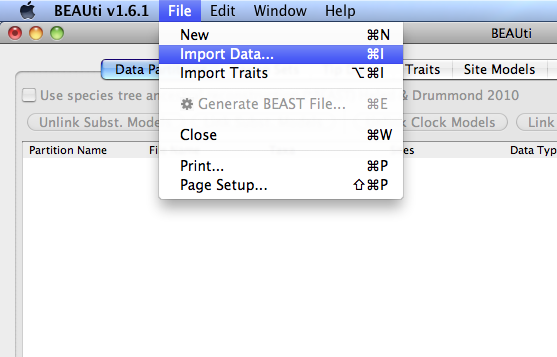
\includegraphics[scale=0.5]{figures/ImportNexus}

\medskip{}

Select the file called \texttt{primates.nex}. This file contains an alignment
of sequences of 12 species of primates. It looks like
this (the lines have been truncated):

\begin{verbatim}
#NEXUS
begin data;
dimensions ntax=12 nchar=898;
format datatype=dna interleave=no gap=-;
matrix
Tarsius_syrichta  AAGTTTCATTGGAGCCACCACTCTTATAATTGCCCATGGCCTCACC
Lemur_catta       AAGCTTCATAGGAGCAACCATTCTAATAATCGCACATGGCCTTACA
Homo_sapiens	     AAGCTTCACCGGCGCAGTCATTCTCATAATCGCCCACGGGCTTACA
Pan               AAGCTTCACCGGCGCAATTATCCTCATAATCGCCCACGGACTTACA
Gorilla           AAGCTTCACCGGCGCAGTTGTTCTTATAATTGCCCACGGACTTACA
Pongo             AAGCTTCACCGGCGCAACCACCCTCATGATTGCCCATGGACTCACA
Hylobates         AAGCTTTACAGGTGCAACCGTCCTCATAATCGCCCACGGACTAACC
Macaca_fuscata    AAGCTTTTCCGGCGCAACCATCCTTATGATCGCTCACGGACTCACC
M_mulatta         AAGCTTTTCTGGCGCAACCATCCTCATGATTGCTCACGGACTCACC
M_fascicularis    AAGCTTCTCCGGCGCAACCACCCTTATAATCGCCCACGGGCTCACC
M_sylvanus        AAGCTTCTCCGGTGCAACTATCCTTATAGTTGCCCATGGACTCACC
Saimiri_sciureus	 AAGCTTCACCGGCGCAATGATCCTAATAATCGCTCACGGGTTTACT
;
end;

begin assumptions;
	charset firsthalf = 1-449;
	charset secondhalf = 450-898;
end;
end;\end{verbatim}

\medskip{}

Once loaded, the two character partitions are displayed in the main panel:

\medskip{}

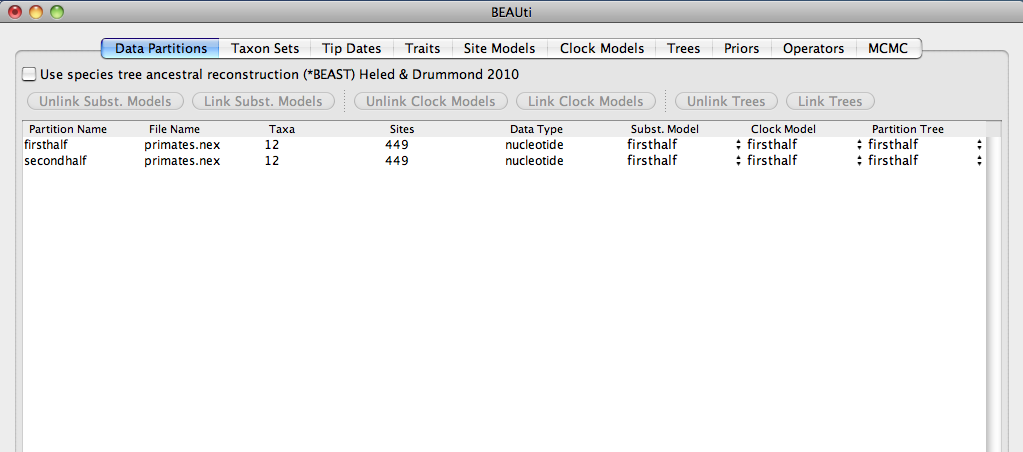
\includegraphics[scale=0.4]{figures/BEAUti_DataPartitions}

\medskip{}

\subsubsection*{Defining the calibration nodes}

Select the {\bf Taxon Sets} tab at the top of the main window. You will see the
panel that allows you to create sets of taxa. Once you have created a taxa set you will be able to add calibration information for its most recent common
ancestor (MRCA) later on. Press the small ``plus''
button at the bottom left of the panel. This will create a new taxon
set. 

Rename it by double-clicking on the entry that appears (it will
initially be called \texttt{untitled1}). Call it \texttt{ingroup} (it will contain all taxa except the lemur, which will form the outgroup).
In the next table along you will see the available taxa. Select all taxa and press the green arrow button. Move the \texttt{Lemur} back into the excluded taxa set. Since we know that lemur is the outgroup, we will set select the checkbox in the \texttt{Monophyletic?} column. This will ensure that the ingroup is kept monophyletic during the course of the MCMC analysis.

Now repeat the whole procedure creating a set called \texttt{Human-Chimp}
that contains only \texttt{Homo\_sapiens} and \texttt{Pan}
taxa. The screen should look like this:

\medskip{}

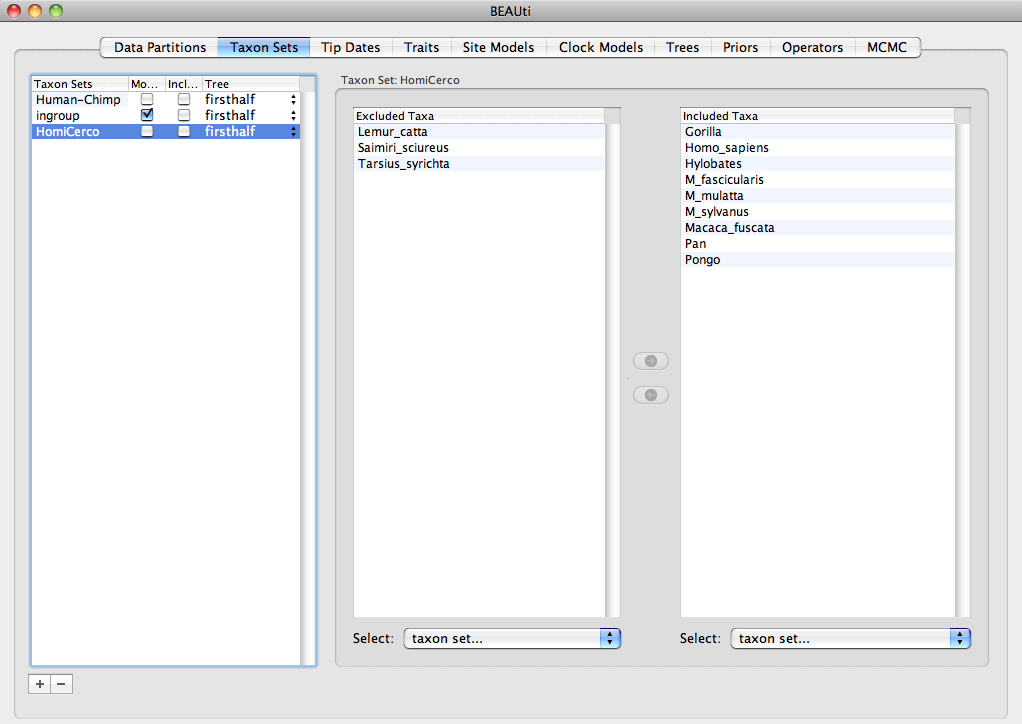
\includegraphics[scale=0.4]{figures/BEAUti_TaxonSets}

\medskip{}


Finally, create a taxon group that contains everything under the hominoid/cercopithecoid split (i.e. everything except \texttt{Lemur}, \texttt{Saimiri} and \texttt{Tarsius}). Call this taxon set something like \texttt{HomiCerco}.

\subsubsection*{Unlink partition models}

At this point we will need to unlink the substitution model so that each parameter is estimated separately for the two partitions. To do this return to {\bf Data Partitions} panel, select both partitions in the table and click the \texttt{Unlink Subst Models} button. 

\medskip{}

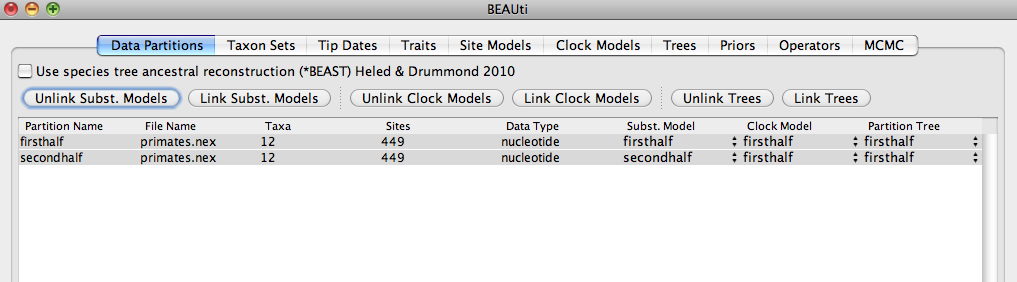
\includegraphics[scale=0.4]{figures/BEAUti_Unlink}

\medskip{}

And you can also change the partition model name in its corresponding panel (e.g. {\bf Clock Models}  panel), and make the final partitions as illustrated below:

\medskip{}

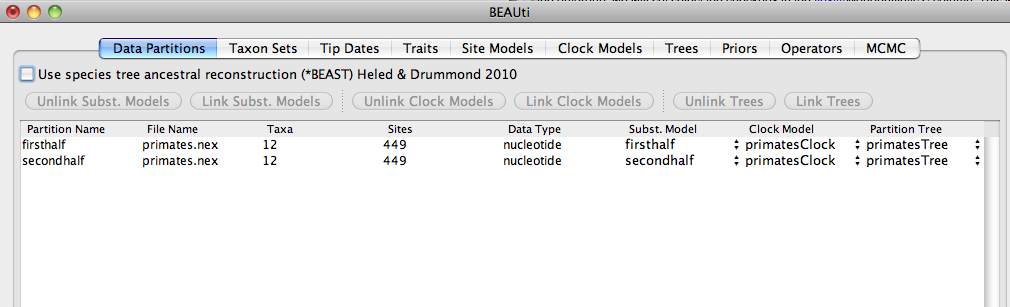
\includegraphics[scale=0.4]{figures/BEAUti_DataPartitions_final}

\medskip{}



\subsubsection*{Setting the substitution model}

The next thing to do is to click on the {\bf Site Models} tab at the top of the
main window. This will reveal the evolutionary model settings for
BEAST. Exactly which options appear depend on whether the data are
nucleotides, or amino acids, or binary data, or general data.
The settings that will appear after loading the Primates data set will
be the default values so we need to make some changes. 

Most of the models should be familiar to you. For this analysis, we
will \underline{respectively} select substitution models listed each time on the 
left side make the same change: select \textbf{Gamma} under the 
\textbf{Site Heterogeneity Model} menu which will allow rate variation 
between sites in the associated alignment. 

\medskip{}

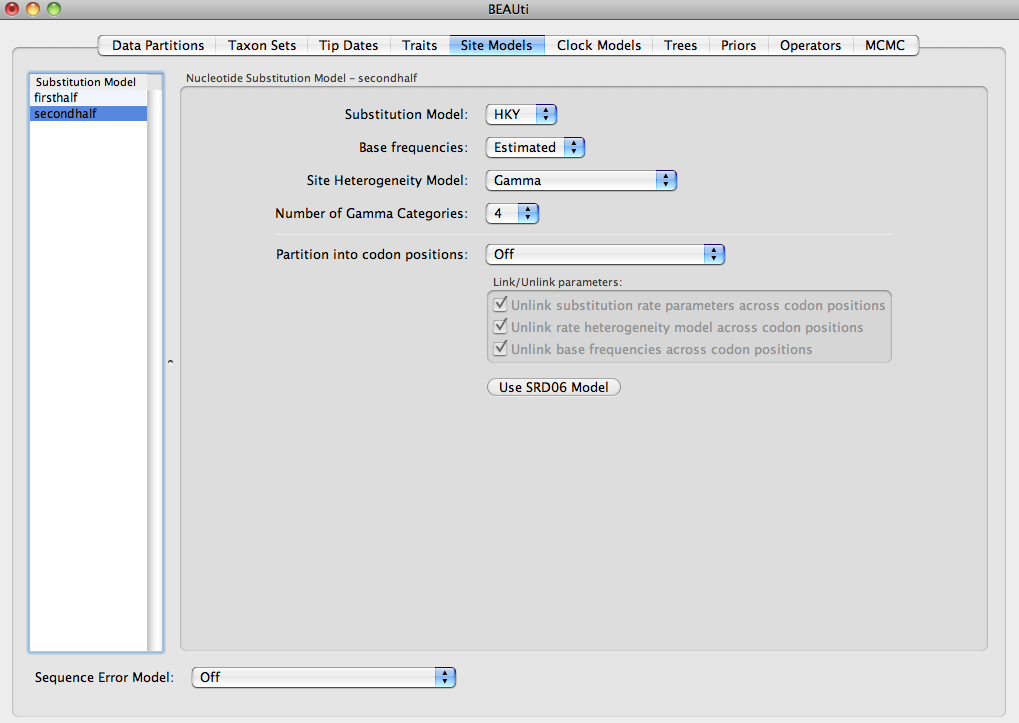
\includegraphics[scale=0.4]{figures/BEAUti_Model}

\medskip{}


\subsubsection*{Setting the clock model}

Second, we will do is to click on the {\bf Clock Models} tab at the top of the
main window, and to change the molecular clock model to \textbf{Relaxed Clock: Uncorrelated
Log-normal} so as to account for lineage-specific rate heterogeneity.
Your model options should now look like this: 

\medskip{}

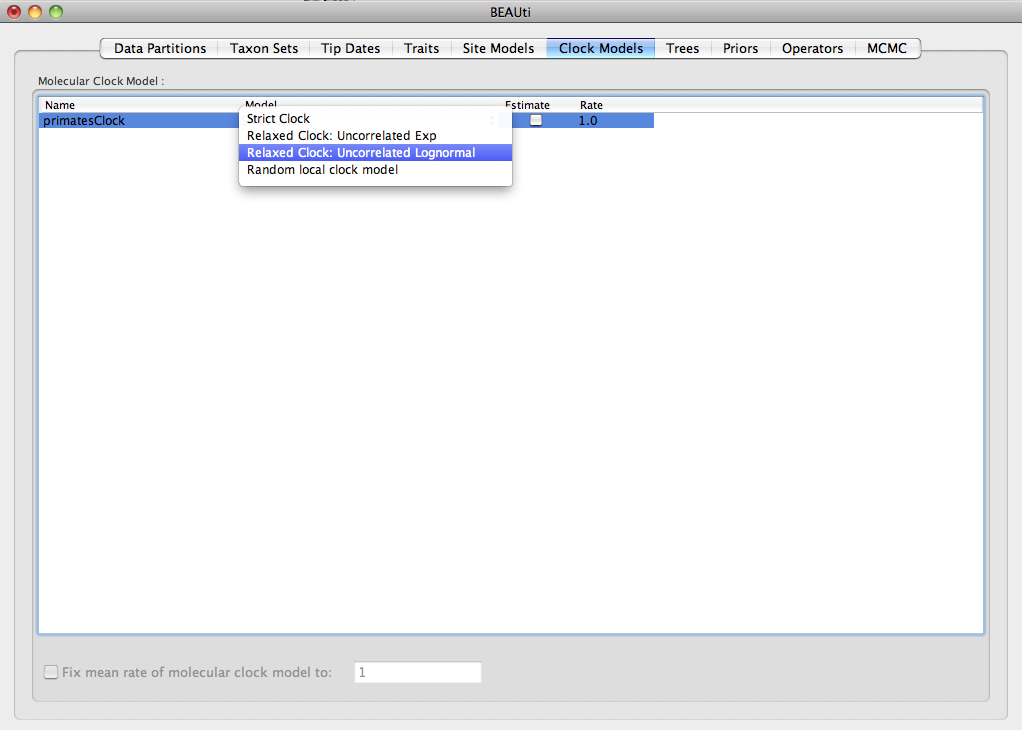
\includegraphics[scale=0.4]{figures/BEAUti_Clock}

\medskip{}

The \textbf{Estimate} check box is required to be checked, because we wish to estimate
the clock rate (and in doing so the divergence times). But this will be automatically checked, in this case, when we put a proper prior on \textbf{tmcra} statistics appeared in \textbf{Priors} panel.

\subsubsection*{Trees }

The {\bf Trees} tab allows priors to be specified for each parameter in the
model. The first thing to do is to specify that we wish to use the \textbf{Yule} model 
as the tree prior. This is a simple model of speciation that
is generally more appropriate when considering sequences from different species.
Select this from the {\bf Tree prior} dropdown menu.

\medskip{}

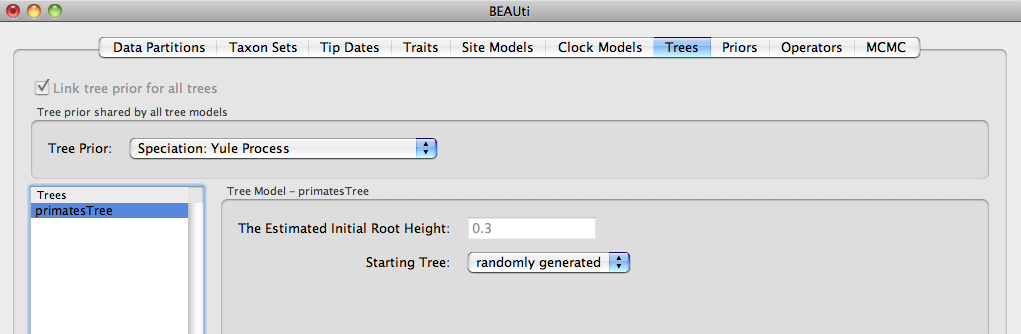
\includegraphics[scale=0.4]{figures/BEAUti_Tree}

\medskip{}

\subsubsection*{Priors }

The {\bf Priors} tab allows priors to be specified for each parameter in the
model. The first thing to do is to specify that we wish to use the Yule model 
as the tree prior. This is a simple model of speciation that
is generally more appropriate when considering sequences from different species.
Select this from the {\bf Tree prior} dropdown menu.

We now need to specify a prior distribution for some of the divergence times, based on our prior fossil knowledge. This is known
as calibrating our tree. We will actually use two calibrations
in this analysis. Click on the button in the table next to \texttt{tmrca(human-chimp)}, A dialog box will appear allowing you to specify a prior for the MRCA of species. 

Select the \textbf{Normal} distribution.
We are going to assume a normal distribution centered at 6 million
years with a standard deviation of 0.5 million years. This will give
a central 95\% range of about 5-7 My. This corresponds to the consensus
estimate of the date of the most recent common ancestor of humans and chimps.

Following the same procedure set a calibration of 24 +/- 0.5 million (stdev) for the hominoid-cercopithecoid split.

Although we created a taxon set for the ingroup (\texttt{tmrca(ingroup)}
in the prior table), we are not going to put an informative prior
on this. We can then estimate this divergence time based on the other calibrations. 

\medskip{}

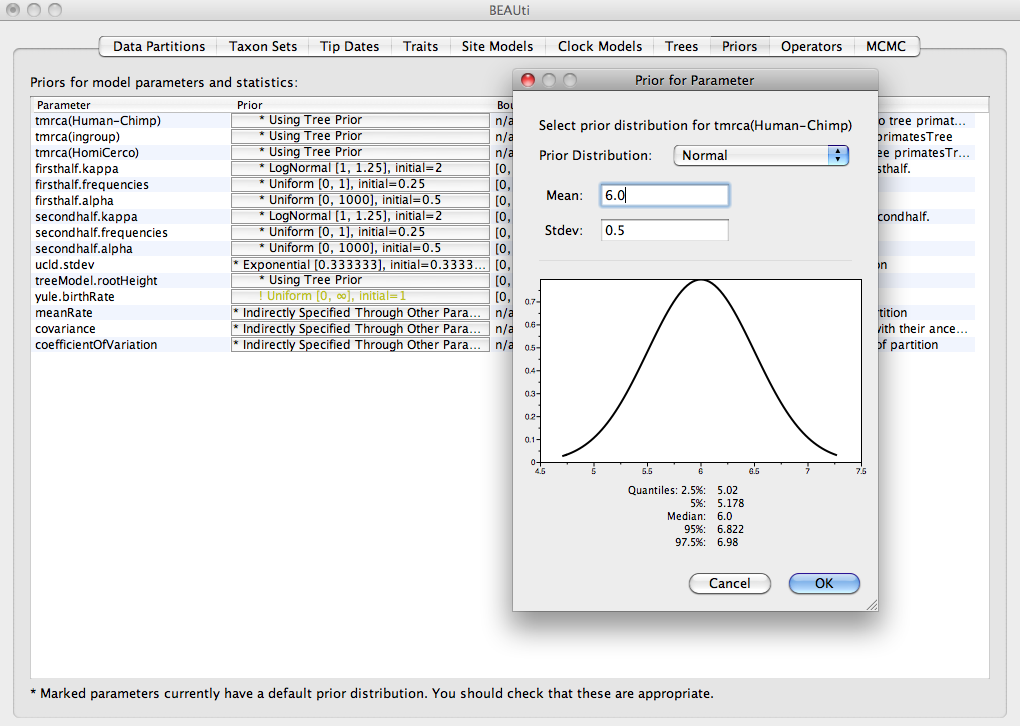
\includegraphics[scale=0.4]{figures/BEAUti_Prior1}

\medskip{}

And the clock model parameters will appear when the clock rate is estimated. The priors table should now look like this: 

\medskip{}

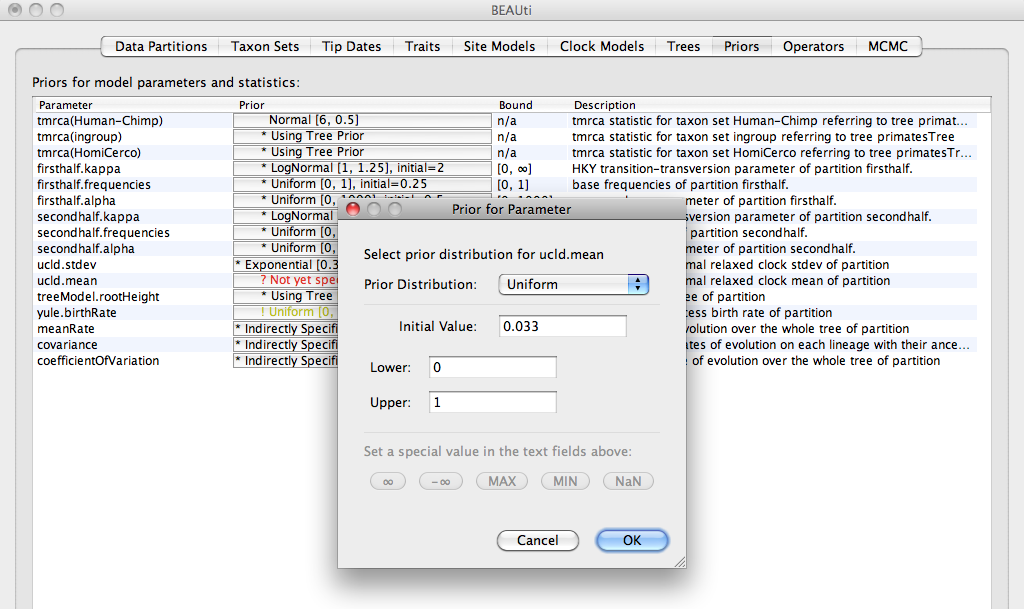
\includegraphics[scale=0.4]{figures/BEAUti_Prior2}

\medskip{}


\subsubsection*{Setting the MCMC options }

Ignore the \textbf{Operators} tab as this just contains technical
settings effecting the efficiency of the MCMC program (see Notes for details). 

The next tab, {\bf MCMC}, provides more general
settings to control the length of the MCMC and the file names. 

Firstly we have the \textbf{Length of chain}. This is the number of
steps the MCMC will make in the chain before finishing. How long this
should be depends on the size of the data set, the complexity of the
model and the quality of answer required. The default value of 10,000,000
is entirely arbitrary and should be adjusted according to the size
of your data set. For this data set let's initially set the chain
length to 800,000 as this will run reasonably quickly on most modern
computers (a few minutes).

\medskip{}

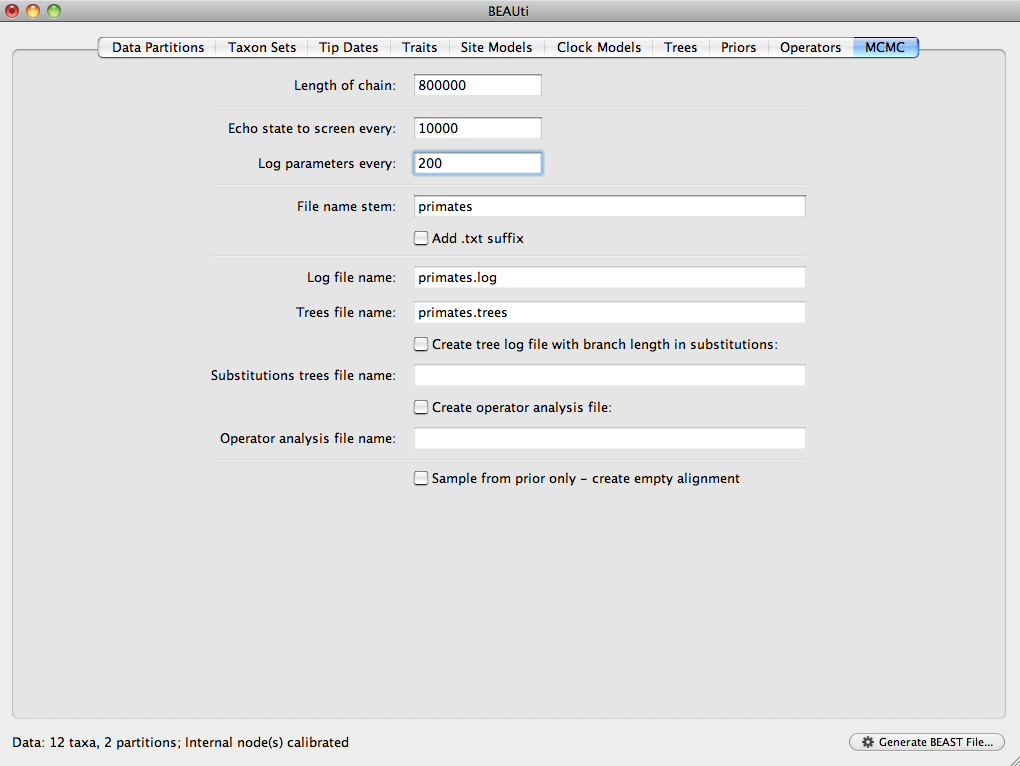
\includegraphics[scale=0.4]{figures/BEAUti_MCMC}

\medskip{}

The next options specify how often the parameter values in the Markov
chain should be displayed on the screen and recorded in the log file.
The screen output is simply for monitoring the programs progress so
can be set to any value (although if set too small, the sheer quantity
of information being displayed on the screen will actually slow the
program down). For the log file, the value should be set relative
to the total length of the chain. Sampling too often will result in
very large files with little extra benefit in terms of the precision
of the analysis. Sample too infrequently and the log file will not
contain much information about the distributions of the parameters. 
You probably want to aim to store no more than 10,000 samples so this should be
set to no less than chain length / 10000.

For this exercise we will set the screen log to 10,000 and the file log to 200. The final two
options give the file names of the log files for the sampled parameters and
the trees. These will be set to a default based on the name of the
imported NEXUS file. 

\begin{itemize}
\item If you are using windows then we suggest you add the suffix \texttt{.txt} to both of these (so,
\texttt{Primates.log.txt} and \texttt{Primates.trees.txt}) so that Windows recognizes
these as text files. 
\end{itemize}

\subsubsection*{Generating the BEAST XML file }

We are now ready to create the BEAST XML file. To do this,
either select the \textbf{Generate BEAST File...} option from the \textbf{File} menu or click the similarly labelled button at the bottom of the
window. Check the default priors, and save the file with an appropriate name
(we usually end the filename with \texttt{.xml}, i.e., \texttt{Primates.xml}).
We are now ready to run the file through BEAST. 

\subsection*{Running BEAST }

\medskip{}

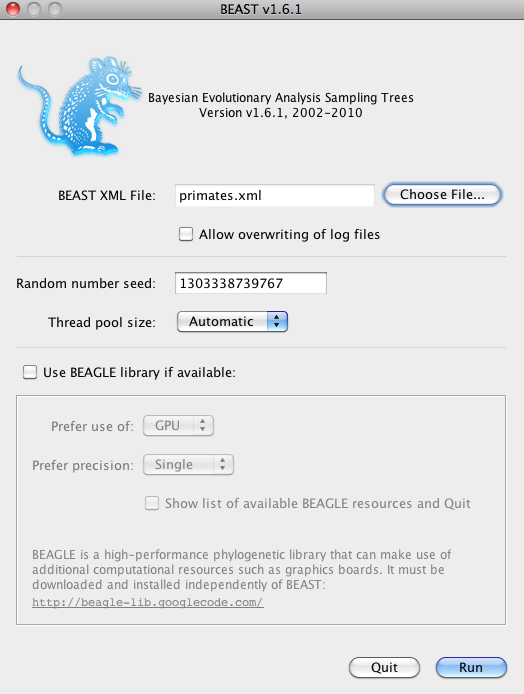
\includegraphics[scale=0.5]{figures/BEAST}

\medskip{}

Now run BEAST and when it asks for an input file, provide your newly
created XML file as input. BEAST will then run until it has finished
reporting information to the screen. The actual results files are
save to the disk in the same location as your input file. The output to the screen will
look something like this: 

{\scriptsize   
\begin{verbatim}

                   BEAST v1.6.1, 2002-2010
       Bayesian Evolutionary Analysis Sampling Trees
                 Designed and developed by
   Alexei J. Drummond, Andrew Rambaut and Marc A. Suchard
                              
               Department of Computer Science
                   University of Auckland
                  alexei@cs.auckland.ac.nz
                              
             Institute of Evolutionary Biology
                  University of Edinburgh
                     a.rambaut@ed.ac.uk
                              
              David Geffen School of Medicine
           University of California, Los Angeles
                     msuchard@ucla.edu
                              
                Downloads, Help & Resources:
                 	http://beast.bio.ed.ac.uk
                              
Source code distributed under the GNU Lesser General Public License:
            	http://code.google.com/p/beast-mcmc
                              
                     BEAST developers:
	Alex Alekseyenko, Erik Bloomquist, Joseph Heled, Sebastian Hoehna, 
	Philippe Lemey, Wai Lok Sibon Li, Gerton Lunter, Sidney Markowitz, 
	Vladimir Minin, Michael Defoin Platel, Oliver Pybus, Chieh-Hsi Wu, Walter Xie
                              
                         Thanks to:
    	Roald Forsberg, Beth Shapiro and Korbinian Strimmer


Random number seed: 1303338739767

Parsing XML file: primates.xml
  File encoding: MacRoman
Read alignment: alignment
  Sequences = 12
      Sites = 898
   Datatype = nucleotide
Site patterns 'firsthalf.patterns' created from positions 1-449 of alignment 'alignment'
  pattern count = 227
Site patterns 'secondhalf.patterns' created from positions 450-898 of alignment 'alignment'
  pattern count = 231
Using Yule prior on tree
Creating the tree model, 'treeModel'
  initial tree topology = ((((((Gorilla,Tarsius_syrichta),Pan),M_sylvanus),(M_mulatta,Macaca_fuscata)),((((Homo_sapiens,Saimiri_sciureus),Pongo),M_fascicularis),Hylobates)),Lemur_catta)
  tree height = 311.73866128365125
Using discretized relaxed clock model.
  over sampling = 1
  parametric model = logNormalDistributionModel
   rate categories = 22
Creating state frequencies model: Initial frequencies = {0.25, 0.25, 0.25, 0.25}
Creating HKY substitution model. Initial kappa = 2.0
Creating site model.
  4 category discrete gamma with initial shape = 0.5
Creating state frequencies model: Initial frequencies = {0.25, 0.25, 0.25, 0.25}
Creating HKY substitution model. Initial kappa = 2.0
Creating site model.
  4 category discrete gamma with initial shape = 0.5
TreeLikelihood(treeModel) using native nucleotide likelihood core
  Ignoring ambiguities in tree likelihood.
  With 227 unique site patterns.
Branch rate model used: discretizedBranchRates
TreeLikelihood(treeModel) using native nucleotide likelihood core
  Ignoring ambiguities in tree likelihood.
  With 231 unique site patterns.
Branch rate model used: discretizedBranchRates
Creating swap operator for parameter branchRates.categories (weight=10.0)
Likelihood is using -1 threads.
Creating the MCMC chain:
  chainLength=800000
  autoOptimize=true
  autoOptimize delayed for 8000 steps
# BEAST v1.6.1, Build r3651
# Generated Thu Apr 21 16:27:15 NZST 2011 [seed=1303338739767]
state	Posterior   	Prior       	Likelihood  	rootHeight  	ucld.mean   
0	-115044.0238	-105244.7369	-9799.2869  	311.739     	3.3E-2      	-
10000	-6019.0942  	-48.1460    	-5970.9482  	31.2013     	1.13161E-2  	-
20000	-5932.1777  	-53.7968    	-5878.3809  	58.3426     	7.80428E-3  	0.11 hours/million states
30000	-5864.1836  	-55.6386    	-5808.5450  	54.7400     	9.7303E-3   	0.09 hours/million states
40000	-5845.2874  	-58.9120    	-5786.3753  	82.1531     	6.86446E-3  	0.08 hours/million states
50000	-5798.2689  	-60.2217    	-5738.0472  	87.4058     	7.84354E-3  	0.08 hours/million states
60000	-5779.7566  	-57.1298    	-5722.6268  	49.1015     	1.17545E-2  	0.07 hours/million states
70000	-5787.4056  	-60.5876    	-5726.8180  	81.5675     	1.03161E-2  	0.07 hours/million states
80000	-5785.8794  	-58.9768    	-5726.9027  	70.4040     	9.80333E-3  	0.07 hours/million states
90000	-5778.6354  	-59.2618    	-5719.3737  	77.9236     	1.0054E-2   	0.07 hours/million states
100000	-5780.4106  	-60.2610    	-5720.1496  	78.7802     	8.80928E-3  	0.07 hours/million states

... ...

790000	-5772.8359  	-59.0540    	-5713.7819  	77.1089     	9.1281E-3   	0.06 hours/million states
800000	-5774.2917  	-57.2419    	-5717.0498  	61.2605     	9.77329E-3  	0.06 hours/million states

Operator analysis
Operator                                          Tuning   Count      Time     Time/Op  Pr(accept)  Performance suggestion
scale(firsthalf.kappa)                            0.536   701        232      0.33     0.2596      good	
firsthalf.frequencies                             0.059   677        206      0.3      0.2851      good	
scale(firsthalf.alpha)                            0.598   719        220      0.31     0.3255      good	
scale(secondhalf.kappa)                           0.555   685        222      0.32     0.3109      good	
secondhalf.frequencies                            0.058   661        216      0.33     0.3238      good	
scale(secondhalf.alpha)                           0.598   680        210      0.31     0.3015      good	
scale(ucld.mean)                                  0.697   21192      7410     0.35     0.2786      good	
scale(ucld.stdev)                                 0.274   21350      7342     0.34     0.3526      good	
subtreeSlide(treeModel)                           4.405   105795     18763    0.18     0.337       good	
Narrow Exchange(treeModel)                                106685     19150    0.18     0.0004      very low	
Wide Exchange(treeModel)                                  21301      2071     0.1      0.0         very low	
wilsonBalding(treeModel)                                  21229      3431     0.16     0.0         very low	
scale(treeModel.rootHeight)                       0.853   21224      1334     0.06     0.218       good	
uniform(nodeHeights(treeModel))                           213114     43645    0.2      0.222       good	
scale(yule.birthRate)                             0.268   21594      697      0.03     0.2761      good	
up:ucld.mean down:nodeHeights(treeModel)          0.596   21448      7551     0.35     0.2417      slightly high	Try setting scaleFactor to about 0.586
swapOperator(branchRates.categories)                      70928      16433    0.23     0.6553      high	No suggestions
randomWalkInteger(branchRates.categories)                 70818      13509    0.19     0.9432      very high	Try increasing windowSize to about 2.0
uniformInteger(branchRates.categories)                    71199      14008    0.2      0.7518      high	

3.028016666666667 minutes 
\end{verbatim}}

\subsection*{Analyzing the results}

Run the program called {\bf Tracer} to analyze the output of BEAST. When the main
window has opened, choose {\bf Import Trace File...} from the {\bf File} menu and select the file that
BEAST has created called \texttt{Primates.log}.
You should now see a window like the following:

\medskip{}

\frame{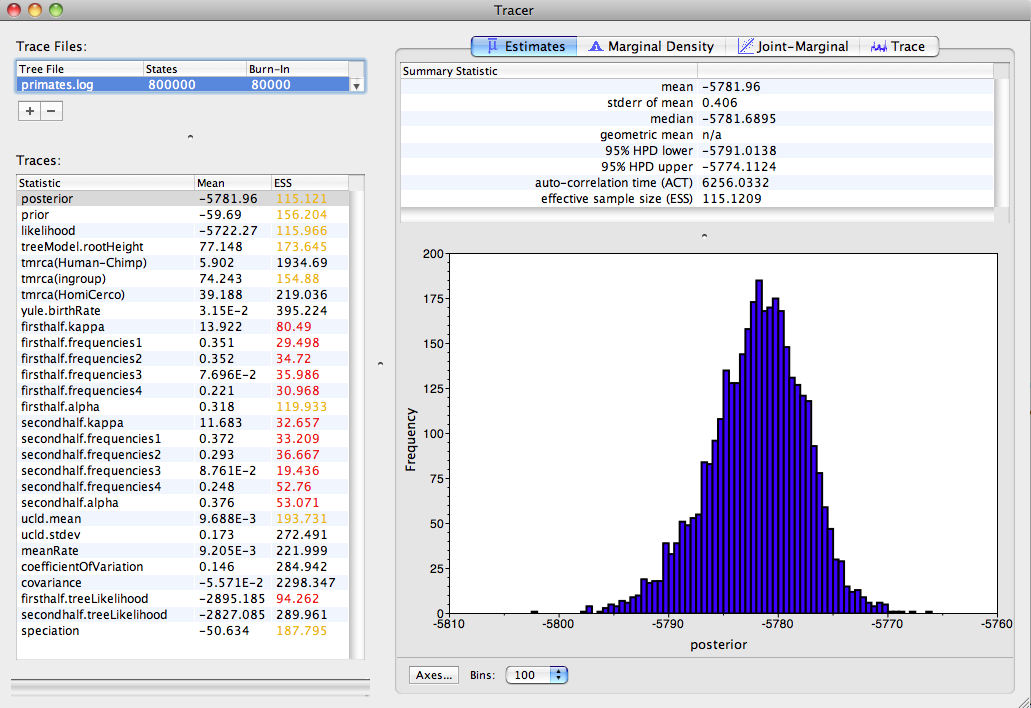
\includegraphics[scale=0.4]{figures/Tracer1}}

\medskip{}

Remember that MCMC is a stochastic algorithm so the actual numbers will not be exactly the same.

On the left hand side is a list of the different quantities that BEAST has logged. 
There are traces for the posterior (this
is the log of the product of the tree likelihood and the prior probabilities), and the continuous parameters. Selecting a trace
on the left brings up analyses for this trace on the right hand side depending on tab that is selected. When first opened, the
`posterior' trace is selected and various statistics of this trace are shown under the Estimates tab.
In the top right of the window is a table of calculated statistics for the selected trace. 

Select \texttt{meanRate} to look at
the rate of evolution averaged over the whole tree. Tracer will plot a (marginal posterior) distribution for the selected parameter and also give you
statistics such as the mean and median. The 95\% HPD stands for {\it highest posterior density interval} and represents the most compact interval on the selected parameter that contains 95\% of the posterior probability. It can be thought of as a Bayesian analog to a confidence interval. 

\newpage
\subsection*{Questions}
 \vspace{5 mm}

\textit{What is the rate of molecular evolution in Primates (include the HPD interval)?}

 \vspace{5 mm}
 \framebox(420,30){}
  \vspace{5 mm}


\textit{What sources of error does this estimate include?}
 
 \vspace{5 mm}
 \framebox(420,60){}
   \vspace{5 mm}
   
   The \texttt{coefficientOfVariation} statistic gives a summary of how much the rate of evolution varies from lineage to lineage (expressed as a proportion of the mean rate).
   
   \bigskip{}

\textit{Does the rate of evolution differ substantially amongst different lineages in the tree?}

 \vspace{5 mm}
 \framebox(420,60){}
   \vspace{5 mm}

Selecting the \texttt{treeModel.rootHeight} parameter gives the marginal posterior distribution of the age of the root of entire tree.

   \bigskip{}

\textit{How old is the root of the tree (give the mean and the HPD range)?}

 \vspace{5 mm}
 \framebox(420,30){}
   \vspace{5 mm}

Select the \texttt{treeModel.rootHeight} parameter and the next three (hold shift whilst selecting). This will show a display of the
age of the root and the three MRCAs we specified in BEAUti. The parameter that we used to calibrate the tree
(\texttt{tmrca(human-chimp)}) will have posterior distributions very similar to the prior distributions
that we specified. 

\medskip{}

\frame{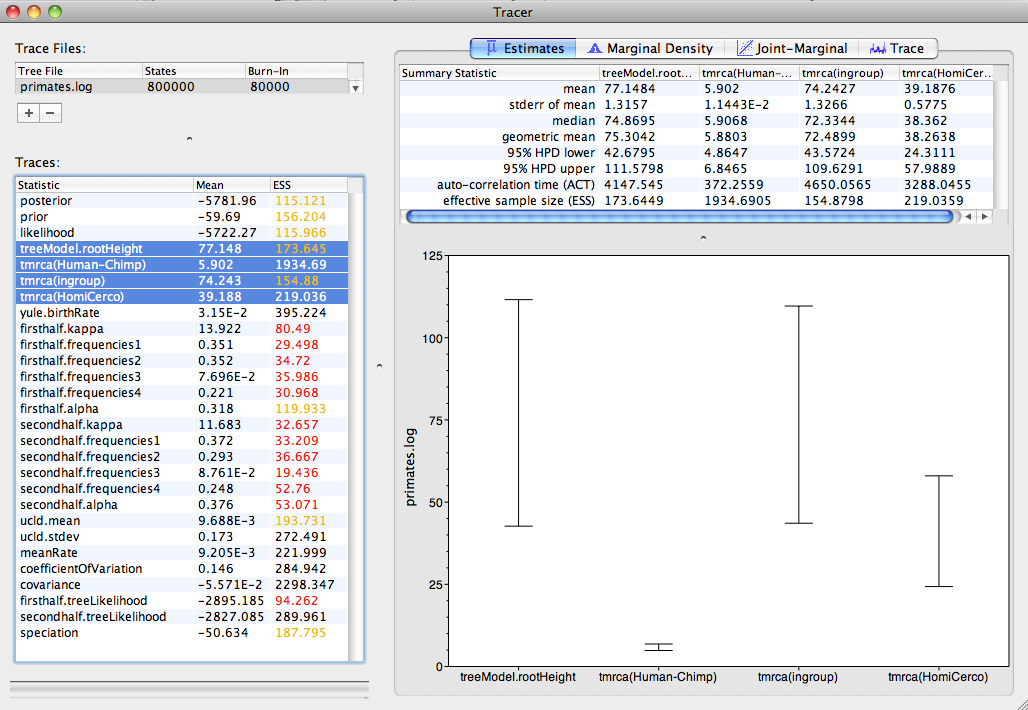
\includegraphics[scale=0.4]{figures/Tracer_divergences}}

\medskip{}

If you switch the tab at the top of the window to {\bf Marginal Density} then you will get a plot of the marginal posterior densities of each of these date estimates overlayed:

\medskip{}

\frame{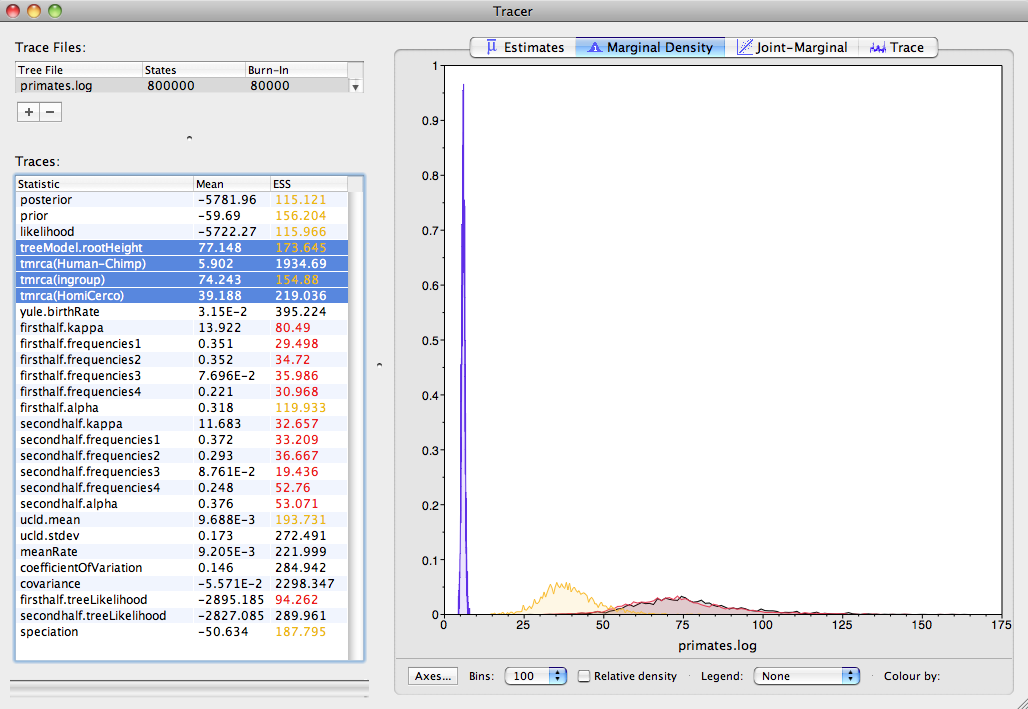
\includegraphics[scale=0.4]{figures/Tracer_marginalDensity}}

\medskip{}

\subsection*{Obtaining an estimate of the phylogenetic tree}

BEAST also produces a sample of plausible trees along with its sample of parameter estimates. 
These need to be summarized
using the program {\bf TreeAnnotator} (see Notes for details). This will take the set of trees and find the best
supported one. It will then annotate this summary tree with the mean ages of all the
nodes and the HPD ranges. It will also calculate the posterior clade probability for each
node. Run the TreeAnnotator program and set it up to look like this:

\medskip{}

\frame{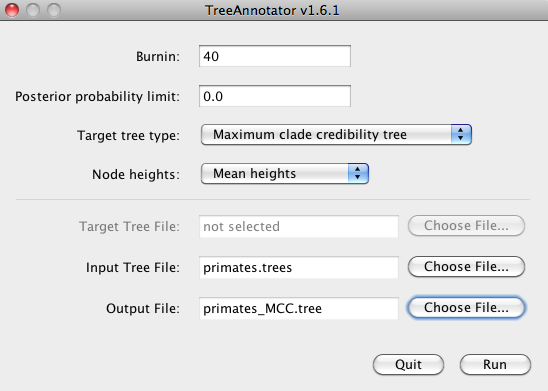
\includegraphics[scale=0.5]{figures/TreeAnnotator1}}

\medskip{}

The burnin is the number of trees to remove from the start of the sample. Unlike {\bf Tracer} which specifies the number of
steps as a burnin, in {\bf TreeAnnotator} you need to specify the actual number of trees. For this run, you specified a chain
length of 800,000 steps sampling every 200 steps. Thus the trees file will contain 4000 trees and so to specify a 1\% burnin
use the value 40.

The {\bf Posterior probability limit} option specifies a limit such that if a node is found at less than this frequency in the sample
of trees (i.e., has a posterior probability less than this limit), it will not be annotated. The default of 0.5 means that only nodes
seen in the majority of trees will be annotated. Set this to zero to annotate all nodes.

For {\bf Target tree type} you can either choose a specific tree from a file or ask TreeAnnotator to find a tree in your sample.
The default option, {\bf Maximum clade credibility tree}, finds the tree with the highest product of the posterior probability of
all its nodes.

Choose {\bf Mean heights} for node heights. This sets the heights (ages) of each node in the tree to the mean height across the
entire sample of trees for that clade.

For the input file, select the trees file that BEAST created (by default this will be called \texttt{Primates.trees}) and select a file for the
output (here we called it \texttt{Primates\_MCC.tree}).

Now press Run and wait for the program to finish.

\subsection*{Viewing the Tree}
Finally, we can look at the tree in another program called {\bf FigTree}. Run this program, and open
the \texttt{Primates.MCC.tree} file by using the Open command in the File menu. The tree should appear.
You can now try selecting some of the options in the control panel on the left. Try selecting
{\bf Node Bars} to get node age error bars. Also turn on {\bf Branch Labels} and select {\bf posterior} to get
it to display the posterior probability for each node. Under {\bf Appearance} you can also tell FigTree
to colour the branches by the rate.
You should end up with something like this:

\medskip{}

\frame{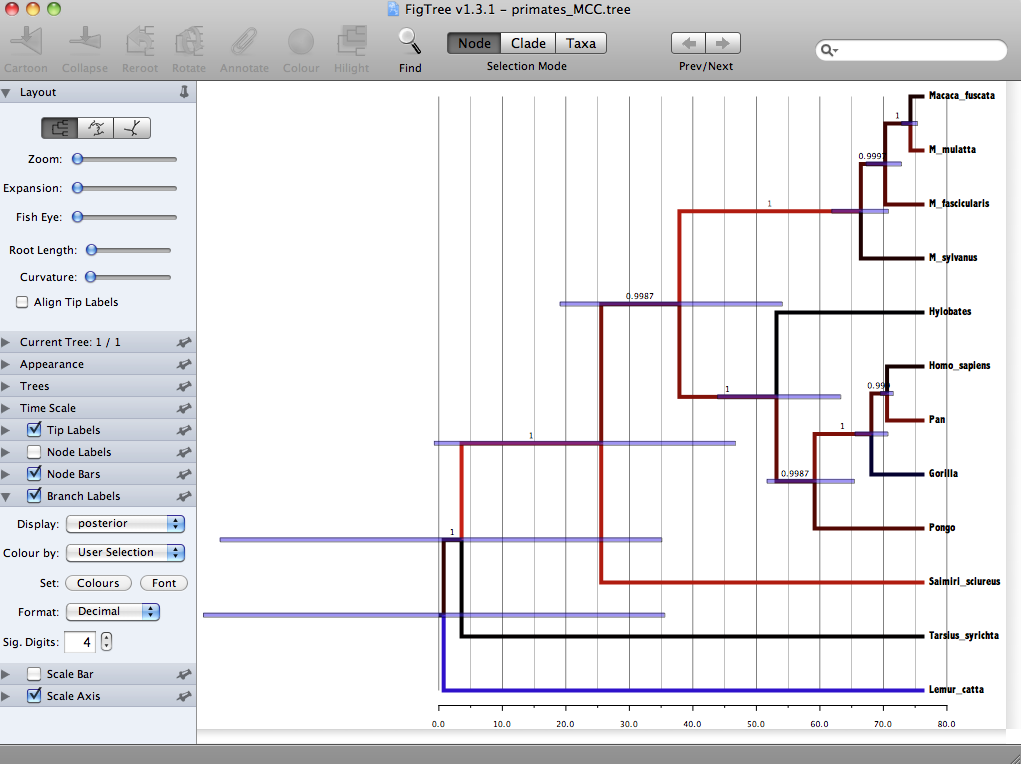
\includegraphics[scale=0.36]{figures/FigTree}}

\medskip{}

\textit{Which branch has the fastest rate of evolution and what is the estimated rate?}

 \vspace{5 mm}
 \framebox(420,30){}
  \vspace{5 mm}


\textit{Which branch has the slowest rate of evolution and what is the estimated rate?}
 
 \vspace{5 mm}
 \framebox(420,30){}
   \vspace{5 mm}

\textit{Are these two rate estimates significantly different? How would you answer this question?}
 
 \vspace{5 mm}
 \framebox(420,60){}
   \vspace{5 mm}


\subsection*{Comparing your results to the prior}

Using BEAUti, set up the same analysis but under the MCMC options, select the {\bf Sample from prior only} option. This will allow you to visualize the full prior distribution in the absence of your sequence data. Summarize the trees from the full prior
distribution and compare the summary to the posterior summary tree.

\end{document}
